\chapter{Introducción}

El cerebro humano es una de las estructuras más complejas que se conocen. La neurociencia moderna
lo estudia cada vez con más frecuencia como una \textit{red}: un conjunto de regiones anatómicas
conectadas entre sí, cuya organización se puede modelar y analizar con las herramientas de la
teoría de grafos~\cite{bullmore2009}. A esta representación se la denomina \textit{connectoma}, y
su estudio se ha convertido en un campo de investigación activo dentro de la neuroimagen, con
aplicaciones que van desde la comprensión de la organización funcional del cerebro sano hasta el
estudio de las alteraciones asociadas a distintas patologías neurológicas.

Este Trabajo Fin de Grado aborda el diseño, desarrollo y despliegue de \textbf{Brain Viz}, una
aplicación web para la visualización 3D interactiva de redes cerebrales. Brain Viz permite cargar
una red modelada como grafo, procesarla en un servicio de \textit{backend} que aplica análisis
básico sobre ella y explorarla de forma interactiva directamente en el navegador, sin necesidad de
instalar software especializado. A lo largo de este capítulo se describen la motivación que impulsa
el proyecto, los objetivos que persigue, un análisis de las herramientas similares existentes y la
estructura del resto de la memoria.

\section{Motivación}

Un connectoma se modela habitualmente como un grafo ponderado donde:

\begin{itemize}
	\item cada \textbf{nodo} representa una región cerebral con unas coordenadas espaciales,
	\item cada \textbf{arista} representa una conexión estructural o funcional entre dos regiones,
	\item el \textbf{peso} de la arista expresa la intensidad o relevancia de esa conexión.
\end{itemize}

La figura~\ref{fig:grafo-ponderado} ilustra este concepto con un pequeño grafo ponderado, en el que
los nodos representan regiones y las aristas, etiquetadas con su peso, representan las conexiones
entre ellas.

\begin{figure}[H]
	\centering
	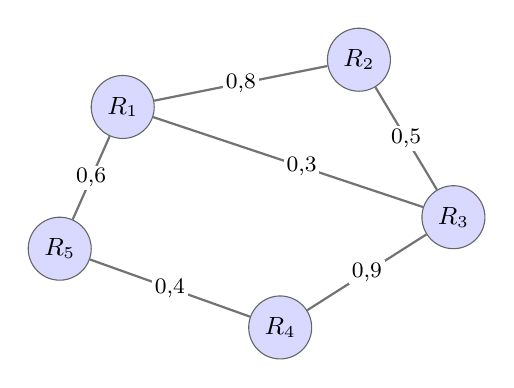
\begin{tikzpicture}[
			every node/.style={font=\small},
			nodo/.style={circle, draw=black!60, fill=blue!15, minimum size=8mm, inner sep=0pt},
			arista/.style={draw=black!55, thick},
			peso/.style={fill=white, inner sep=1pt, font=\footnotesize}]
		\node[nodo] (A) at (0,2)      {$R_1$};
		\node[nodo] (B) at (3,2.6)    {$R_2$};
		\node[nodo] (C) at (4.2,0.6)  {$R_3$};
		\node[nodo] (D) at (2,-0.8)   {$R_4$};
		\node[nodo] (E) at (-0.8,0.2) {$R_5$};
		\draw[arista] (A) -- (B) node[peso, midway] {0,8};
		\draw[arista] (B) -- (C) node[peso, midway] {0,5};
		\draw[arista] (A) -- (C) node[peso, pos=0.55] {0,3};
		\draw[arista] (C) -- (D) node[peso, midway] {0,9};
		\draw[arista] (A) -- (E) node[peso, midway] {0,6};
		\draw[arista] (D) -- (E) node[peso, midway] {0,4};
	\end{tikzpicture}
	\caption[Ejemplo de grafo ponderado.]{Ejemplo de grafo ponderado: los nodos ($R_i$) representan regiones cerebrales y las
	aristas, con su peso asociado, las conexiones entre ellas.}
	\label{fig:grafo-ponderado}
\end{figure}

Trabajar con estos datos no es sencillo. Un connectoma, incluso de tamaño moderado, puede contener
decenas de regiones y cientos o miles de conexiones~\cite{bullmore2009}, de modo que su
interpretación a partir de la matriz de adyacencia en bruto resulta prácticamente inabordable para
una persona. La visualización
se convierte, por tanto, en una herramienta imprescindible: representar la red en el espacio permite
reconocer patrones, identificar regiones especialmente conectadas y comparar unas redes con otras de
un vistazo.

Sin embargo, la combinación de una alta densidad de conexiones con una representación espacial en
tres dimensiones introduce dificultades claras para el análisis visual: oclusión entre elementos,
sobrecarga perceptiva y pérdida de contexto al navegar. Una buena herramienta no solo debe dibujar
la red, sino ofrecer mecanismos de filtrado, resaltado y navegación que permitan reducir esa
complejidad sin ocultar la información relevante.

A esta dificultad técnica se suma una barrera de accesibilidad. Buena parte de las herramientas de
referencia para este tipo de visualización son aplicaciones de escritorio que requieren entornos de
instalación complejos (por ejemplo, dependencias de MATLAB), licencias comerciales o conocimientos
técnicos previos. Esto las aleja de un uso rápido y las hace difíciles de compartir o de reproducir
en equipos distintos.

Surge así la motivación de este trabajo: ofrecer una herramienta \textbf{web} a la que el usuario
acceda desde cualquier navegador moderno, sin tener que instalar nada y sea cual sea el aparato que
tenga a mano, y que le permita visualizar y explorar redes cerebrales sin esperas, manteniendo un equilibrio entre fidelidad de los
datos, rendimiento gráfico y simplicidad de interacción. Al tratarse de una aplicación web, la parte
con la que interactúa el usuario se ejecuta en su navegador, mientras que el procesamiento y el
análisis de las redes se realizan en un servicio de servidor, con lo que la herramienta puede
utilizarse tanto con fines de investigación como docentes, sin barreras de instalación para el
usuario. Además, el proyecto es una oportunidad para trabajar con un \textit{stack} tecnológico
moderno de desarrollo web y visualización 3D, así como con técnicas de contenedorización que
garantizan un despliegue reproducible en cualquier entorno.

\section{Objetivos}

El objetivo general del proyecto es \textbf{diseñar, desarrollar y desplegar Brain Viz, una
aplicación web para la visualización 3D interactiva de redes cerebrales}, obtenidas a partir de
matrices de adyacencia disponibles en bases de datos públicas de neuroimagen. Este objetivo general
se concreta en los siguientes objetivos específicos:

\begin{enumerate}
	\item La aplicación debe permitir \textbf{cargar y visualizar en 3D redes cerebrales} de forma
		interactiva y en tiempo real desde el navegador.
	\item La aplicación debe \textbf{proporcionar un análisis básico} de las métricas fundamentales
		de teoría de grafos de la red.
	\item La aplicación debe ofrecer una \textbf{visualización interactiva} que permita al usuario
		navegar, filtrar, seleccionar e inspeccionar la red con facilidad.
	\item La aplicación debe ser \textbf{fácilmente mantenible y escalable}, con una separación clara
		entre el procesamiento de los datos y su visualización.
	\item La aplicación debe poder \textbf{desplegarse de manera sencilla}, garantizando la
		reproducibilidad del entorno.
\end{enumerate}

Para alcanzar estos objetivos se sigue una metodología de desarrollo ágil basada en
\textit{sprints}, que permite ir entregando versiones funcionales de la aplicación de forma
incremental y validarlas paso a paso.

El sistema se estructura según un modelo cliente-servidor: la parte de visualización se ejecuta en el
navegador del usuario y el procesamiento y análisis de los datos se realizan en un servicio de
servidor, quedando ambos claramente separados y empaquetados en contenedores para facilitar su
despliegue. Cada uno de los objetivos anteriores se irá materializando a lo largo de los distintos
\textit{sprints} descritos en el capítulo de desarrollo.

\section{Descripción de webs similares y sus limitaciones}

Antes de definir la solución se han estudiado varias herramientas existentes para la visualización
de redes cerebrales, con el fin de identificar buenas prácticas y, sobre todo, las limitaciones que
este proyecto pretende resolver. Las referencias más próximas a Brain Viz son dos aplicaciones que
se ejecutan directamente en el navegador, sin instalación, y que confirman la viabilidad e interés
de visualizar connectomas en 3D como una aplicación web.

\textbf{Vizaj}~\cite{vizaj} es una herramienta web libre y de código abierto (desarrollada por el
equipo Inria-NERV) para la visualización interactiva en 3D de redes espaciales, orientada
especialmente a la conectividad cerebral. Está construida con Three.js y se ejecuta por completo en
el navegador. Permite cargar las coordenadas de los nodos y la matriz de conectividad (en formatos
CSV o JSON), ajustar mediante un umbral la densidad de conexiones mostradas, personalizar la
apariencia de los nodos (radio, opacidad y color) y de las aristas, aplicar distintos mapas de color
y mallas de referencia (corteza, cráneo o esfera), y exportar la escena como imagen o como modelo
3D. Es, por tanto, una referencia muy cercana en cuanto a la visualización. Su principal limitación,
desde el punto de vista de este proyecto, es que se trata de una aplicación que se ejecuta
íntegramente en el cliente: se centra en la representación visual y no dispone de un servicio de
\textit{backend} que realice el análisis de la red (métricas de teoría de grafos) ni de una
arquitectura pensada para el despliegue reproducible mediante contenedores.

El \textbf{Connectivity Viewer} de \textbf{BioImage Suite Web}~\cite{bisweb} forma parte de una
completa suite web de análisis de neuroimagen (una adaptación al navegador de la herramienta de
escritorio BioImage Suite), construida con JavaScript, WebGL y WebAssembly. Este módulo permite
cargar matrices de conectividad y representarlas como una red sobre una referencia anatómica del
cerebro; al eliminar también la barrera de la instalación, evidencia el interés de llevar este tipo
de análisis al navegador. Su limitación principal es la opuesta a la de una herramienta ligera: el
visor de conectividad es solo uno de los numerosos módulos de una suite amplia y de propósito
general, orientada al análisis completo de imagen médica, lo que implica una mayor complejidad y una
curva de aprendizaje más pronunciada para quien únicamente desea cargar y explorar un connectoma de
forma inmediata.

\textbf{Neuroglancer}~\cite{neuroglancer}, desarrollado por Google, es otro visor que funciona en el
navegador, en su caso para conjuntos de neuroimagen de gran tamaño, con volúmenes y reconstrucciones
tridimensionales. Su enfoque es distinto al de este trabajo: está pensado para recorrer imágenes y
segmentaciones, no para representar una red de regiones y sus conexiones, y ponerlo en marcha con
datos propios exige familiarizarse con su formato de configuración.

Además de las referencias web anteriores, existen potentes herramientas de escritorio como
\textbf{BrainNet Viewer}~\cite{brainnet}, muy utilizada para la visualización de connectomas y de la
que se adopta en este proyecto el formato de ficheros \texttt{.node} y \texttt{.edge}; su principal
inconveniente es que depende de MATLAB, un entorno comercial. En el ámbito específico de la conectividad,
\textbf{Connectome Workbench}~\cite{workbench} es la herramienta de referencia del Human Connectome
Project para visualizar superficies y datos de conectividad, muy completa pero con instalación
propia, formatos específicos y una curva de aprendizaje considerable para quien solo quiere abrir un
connectoma y mirarlo. Igualmente existen herramientas genéricas de análisis de grafos, como
\textbf{Gephi}~\cite{gephi}, muy potentes en métricas y
algoritmos de disposición, pero no orientadas a datos cerebrales ni a la colocación de los nodos en
sus coordenadas anatómicas reales.

De este análisis se extraen las carencias y oportunidades que Brain Viz pretende cubrir. Frente a
los visores que se ejecutan únicamente en el cliente, Brain Viz adopta una \textbf{arquitectura
cliente-servidor desacoplada}, con un \textit{backend} que analiza la red y expone los resultados a
través de una API, y un despliegue mediante contenedores que garantiza la reproducibilidad. Frente a
las suites complejas de propósito general, Brain Viz es una \textbf{herramienta ligera y enfocada}
específicamente en cargar, explorar y analizar un connectoma de forma inmediata. Buena parte de los
requisitos funcionales del sistema (carga de la red, visualización 3D, navegación, filtrado por
umbral, inspección de nodos, cálculo de métricas y personalización visual) se han extraído de las
funcionalidades observadas en estas herramientas y se detallan y priorizan en el capítulo de
requisitos.

\section{Estructura de la memoria del TFG}

El resto de la memoria se organiza en los siguientes capítulos:

\begin{itemize}
	\item \textbf{Capítulo 2: Requisitos del Software.} Especifica los requisitos funcionales,
		no funcionales y de información, el perfil de usuarios, los casos de uso y los criterios
		de validación del sistema.
	\item \textbf{Capítulo 3: Plan del proyecto.} Describe los recursos (humanos y materiales),
		la planificación temporal, el análisis de las tecnologías disponibles y la estimación de
		costes.
	\item \textbf{Capítulo 4: Desarrollo del software.} Presenta el análisis de arquitecturas y
		patrones y el desarrollo de los distintos \textit{sprints}, incluyendo para cada uno el
		diseño de la interfaz, de los datos y del software, así como su implementación y sus pruebas.
	\item \textbf{Capítulo 5: Manual de instalación.} Detalla los requisitos previos, el
		procedimiento para ejecutar la aplicación en local mediante contenedores y el despliegue en
		un servidor público, junto con la configuración que este requiere.
	\item \textbf{Capítulo 6: Manual de usuario.} Explica cómo utilizar la aplicación, organizado
		según lo que puede hacer cada perfil de usuario.
	\item \textbf{Capítulo 7: Conclusiones.} Recoge la experiencia personal y las propuestas de
		mejora y trabajo futuro.
\end{itemize}
